%----------------------------------------------------------------------------------------
%	PACKAGES AND OTHER DOCUMENT CONFIGURATIONS
%----------------------------------------------------------------------------------------

\documentclass[twoside,twocolumn,a4paper]{article}

\usepackage{blindtext} % Package to generate dummy text throughout this template 

\usepackage[T1]{fontenc} % Use 8-bit encoding that has 256 glyphs
\usepackage{lmodern}

\usepackage{graphicx}

\linespread{1.05} % Line spacing - Palatino needs more space between lines
\usepackage{microtype} % Slightly tweak font spacing for aesthetics

\usepackage[spanish]{babel} % Language hyphenation and typographical rules

\usepackage[numbib,notlof,notlot,nottoc]{tocbibind} % Shows bibliography as a section

\usepackage[hmarginratio=1:1,top=32mm,columnsep=20pt]{geometry} % Document margins

\usepackage[hang, small,labelfont=bf,up,textfont=up]{caption} % Custom captions under/above floats in tables or figures

\usepackage{booktabs} % Horizontal rules in tables

\usepackage{enumitem} % Customized lists

\setlist[itemize]{noitemsep} % Make itemize lists more compact

\usepackage{abstract} % Allows abstract customization

\renewcommand{\abstractnamefont}{\normalfont\bfseries} % Set the "Abstract" text to bold

\usepackage{fancyhdr} % Headers and footers
\pagestyle{fancy} % All pages have headers and footers
\fancyhead{} % Blank out the default header
\fancyfoot{} % Blank out the default footer
\fancyhead[C]{Laboratorio 3 $\bullet$ Informe 1 $\bullet$ Grupo 8: Inafuku, Petino, Poggi} % Custom header text
\fancyfoot[C]{\thepage} % Custom footer text

\usepackage{titling} % Customizing the title section

\usepackage{hyperref} % For hyperlinks in the PDF

%----------------------------------------------------------------------------------------
%	TITLE SECTION
%----------------------------------------------------------------------------------------

\setlength{\droptitle}{-4\baselineskip} % Move the title up

\pretitle{\begin{center}\LARGE\bfseries} % Article title formatting
\posttitle{\end{center}} % Article title closing formatting
\title{Medici\'on de la resistencia de una l\'ampara incandescente} % Article title
\author{%
\textsc{Maximiliano Inafuku} \\[1ex] % Your name
\normalsize \href{mailto:maxi-46@hotmail.com}{maxi-46@hotmail.com} % Your email address
\and % Uncomment if 2 authors are required, duplicate these 4 lines if more
\textsc{Ernesto Petino} \\[1ex] % Second author's name
\normalsize \href{mailto:ernesto.atmo@gmail.com}{ernesto.atmo@gmail.com} % Second author's email address
\and % Uncomment if 2 authors are required, duplicate these 4 lines if more
\textsc{Ignacio Poggi} \\[1ex] % Second author's name
\normalsize \href{mailto:ignaciop.3@gmail.com}{ignaciop.3@gmail.com} % Second author's email address
}

\date{Grupo 8 - Laboratorio 3, C\'atedra Bilbao - Departamento de F\'isica, Facultad de Ciencias Exactas y Naturales, Universidad de Buenos Aires \newline \\ \today} % Leave empty to omit a date
\renewcommand{\maketitlehookd}{%
\begin{abstract}
\noindent En este trabajo se arm\'o un circuito electr\'onico simple para medir la resistencia de una l\'ampara incandescente. Se caracterizaron las resistencias internas de la fuente, volt\'imetro y amper\'imetro utilizados en dicho circuito. Se analizaron los datos obtenidos con el programa Origin y se encontr\'o que la correspondiente a la l\'ampara se ve afectada por la temperatura de su filamento y por la del ambiente.
\end{abstract}
}

%----------------------------------------------------------------------------------------

\begin{document}

% Print the title
\maketitle

%----------------------------------------------------------------------------------------
%	ARTICLE CONTENTS
%----------------------------------------------------------------------------------------

\section{Introducci\'on}

La corriente en un conductor viene dada por un campo el\'ectrico $\mathbf{\vec{E}}$ dentro del conductor que ejerce una fuerza $q\mathbf{\vec{E}}$ sobre las cargas libres. Dichas cargas circulan por el conductor conducidas por las fuerzas debidas al campo el\'ectrico. En un metal, las cargas libres al ser negativas, se mueven en direcci\'on opuesta a $\mathbf{\vec{E}}$ que al interactuar con los iones del material utilizado como conductor, producen fuerzas que se oponen a su movimiento.\par
Como el campo el\'ectrico est\'a siempre dirigido desde las regiones de mayor potencial hacia las de menor potencial, y adem\'as consideramos la corriente como un flujo de cargas positivas, las mismas se mueven en la direcci\'on y el sentido en el que el potencial decrece. Por lo tanto, la diferencia de potencial $V$ entre los puntos $a$ y $b$ (mayor y menor potencial, respectivamente) es \cite{eq:potencial}:
\begin{equation}
\label{eq:potencial}
V = V_{a} - V_{b} = E\Delta L
\end{equation}
donde $\Delta L$ es la longitud de un segmento arbitrario por donde circula la corriente $I$.
\par El cociente entre la ca\'ida de potencial en la direcci\'on de la corriente y la intensidad de \'esta \'ultima se denomina \textbf{resistencia} del segmento \cite{eq:ohm1}:
\begin{equation}
\label{eq:ohm1}
R = \frac{V}{I}
\end{equation}
\par Para muchos materiales, la resistencia no depende de la ca\'ida de voltaje ni de la intensidad. Estos materiales se denominan \'ohmicos, y su caracter\'istica a destacar es que la ca\'ida de potencial a trav\'es de un conductor es proporcional a la corriente (relaci\'on lineal).
\par En estos materiales, $R$ permanece aproximadamente constante, en otros casos (materiales no \'ohmicos) puede variar dependiendo de caracter\'isticas f\'isicas intensivas del material o del entorno (como la temperatura, humedad, etc.). Esta relaci\'on se conoce como la \textit{Ley de Ohm} y se escribe normalmente como \cite{eq:ohm2}:
\begin{equation}
\label{eq:ohm2}
V = IR
\end{equation}
\par En este trabajo veremos como var\'ia la resistencia de la l\'ampara incandescente en funci\'on de la intensidad de corriente circulando en el circuito; teniendo en cuenta la temperatura del filamento y la del ambiente


%------------------------------------------------

\section{Dispositivo experimental}

Los instrumentos de laboratorio utilizados fueron:
\begin{itemize}
\item 
\label{Fuente} Fuente de corriente continua, Hantek PPS-2320A (R\'otulo: FC-04)
\cite{Fuente}
\item 
\label{amp} Mult\'imetro Protek 506, utilizado como amper\'imetro (R\'otulo: 4)
\cite{amp}
\item 
\label{volt} Mult\'imetro UNI-T UT55, utilizado como volt\'imetro (R\'otulo: 2)
\cite{volt}
\item L\'ampara incandescente
\end{itemize}

Para lograr hallar la resistencia de la l\'ampara incandescente fue necesario medir la ca\'ida de potencial y la corriente que circulaba por esta. Para ello se coloc\'o en serie la l\'ampara incandescente y el amper\'imetro y conectados a estos en paralelo el volt\'imetro y la fuente de corriente continua (Figura \ref{fig:dsp_exp}).\par

\begin{figure}[h]
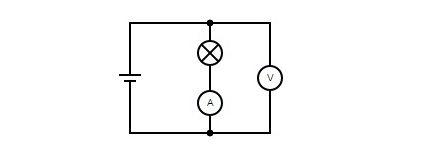
\includegraphics[width=\linewidth]{dispositivo_experimental.jpg}
\caption{Esquema del circuito realizado.}
\label{fig:dsp_exp}
\end{figure}

Se realizaron luego las mediciones, variando la diferencia de potencial de la fuente de corriente continua y tomando los datos de la corriente que pasaba por el amper\'imetro. Debido a que las mediciones se ve\'ian considerablemente afectadas por el ambiente externo (ya que la temperatura afectaba la resistencia, y por ende la corriente) fue necesario aislar de forma parcial a la l\'ampara del medio ambiente. Para ello se coloc\'o una cobertura pl\'astica que cubr\'ia a la misma. Luego, para cada medici\'on de intensidad se esper\'o a que se estabilizara la temperatura de la l\'ampara.

%------------------------------------------------
%------------------------------------------------
\section{Resultados y an\'alisis}

Con los datos obtenidos se grafic\'o la diferencial de potencial registrada por el volt\'imetro en funci\'on de la intensidad. Luego se realizaron un ajuste lineal (Figura \ref{fig:line}), uno de orden dos con el origen forzado (Figura 3), uno de orden dos con los par\'ametros libres (Figura 4) y finalmente uno de orden tres.\par

\begin{figure}[h]
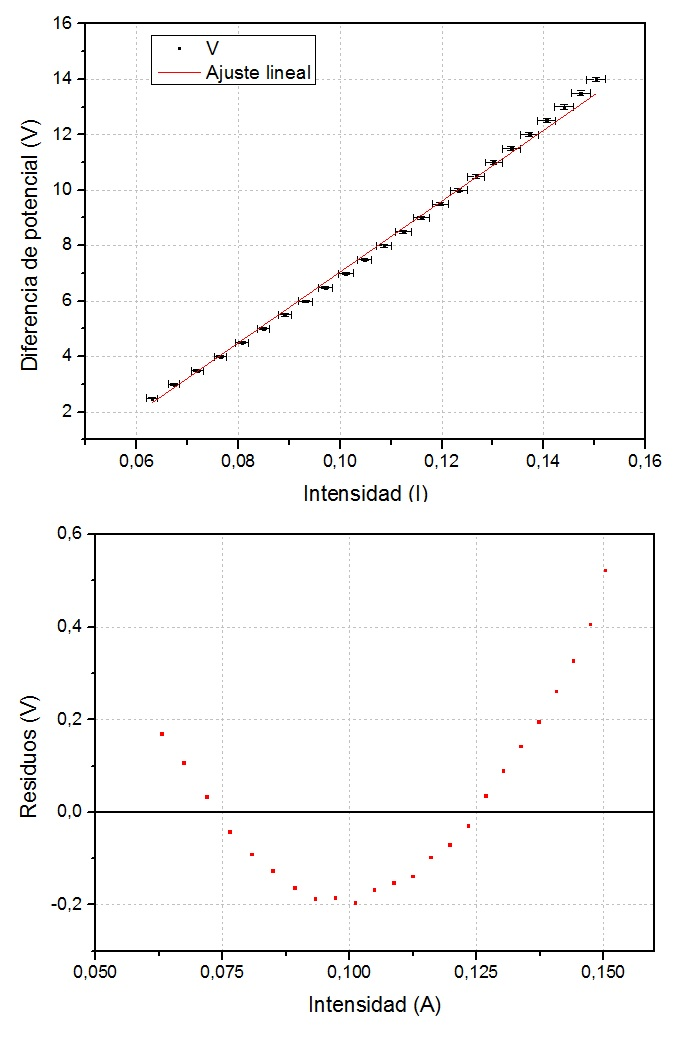
\includegraphics[width=\linewidth]{fig_line.jpg}
\caption{Ajuste lineal y sus residuos}
\label{fig:line}
\end{figure}

\begin{table}[h]
\centering
\caption{Par\'ametros del ajuste lineal}
\label{tab:line}
\begin{tabular}{|c|c|c|c|}
\hline
\multicolumn{4}{|c|}{$y(x)=ax+b$}           \\ \hline
b (V)        & T-valor & a($\Omega$) & T-valor \\ \hline
$-5.7\pm0.1$ & -45     & $128\pm1$   & 94      \\ \hline
\end{tabular}
\end{table}

El ajuste lineal explica la mayor parte de los datos ($R^2=0.9974$), la media de los residuos es cero y el valor del test F es muy elevado ($F-valor=8778$), indicando que es poco probable que el ajuste lineal sea azaroso. Sin embargo, observando el gr\'afico de los residuos (Figura \ref{fig:line}) se puede ver que este modelo no es el m\'as ideal. De hecho es posible notar una fuerte dependencia, similar a una cuadr\'atica, de los residuos en func\'ion de la intensidad. Por estos motivo se realz\'o el ajuste cuadr\'atico con la ordenada forzada en cero(Figura \ref{fig:o2cero}).\par
Adem\'as, considerando la Ley de Ohm, la ordenada al origen del ajuste lineal deber\'ia ser nula. Sin embargo no se observa este comportamiento y el T-valor (Tabla \ref{tab:line}) sugiere que la ordenada de hecho no es nula. Debido a esto, se podr\'ia considerar que en el caso de la l\'ampara incandescente, el modelo simple de la Ley de Ohm no es aplicable de forma directa, sino que habr\'a que considerar el efecto de la temperatura.

%----------ORDEN 2 CERO FORZADO---------------

\begin{table}[h]
\centering
\caption{Par\'ametros del ajuste de orden dos con el cero forzado}
\label{tab:o20}
\begin{tabular}{|c|c|c|c|}
\hline
\multicolumn{4}{|c|}{$y(x)=ax^2+bx$}   \\ \hline
b($\Omega$)& T-valor & a($\Omega/A$) & T-valor \\ \hline
$6\pm2$	   & 3.6     & $600\pm17$    & 36     \\ \hline
\end{tabular}
\end{table}

\begin{figure}[h!]
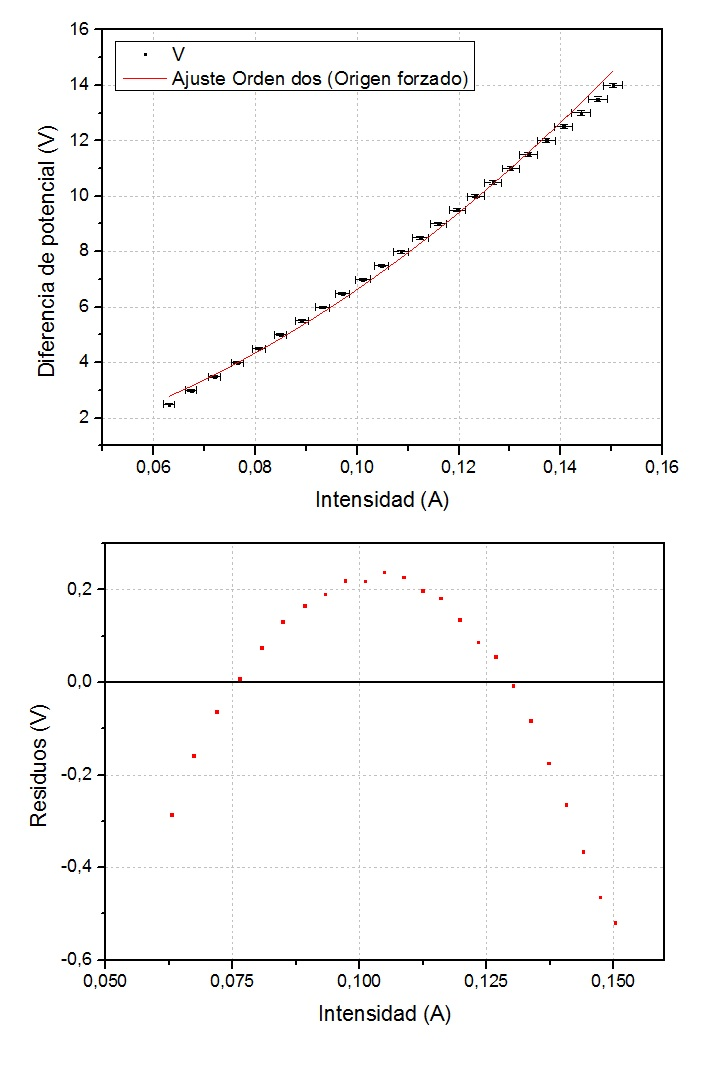
\includegraphics[width=\linewidth]{fig_o2cero.jpg}
\caption{Ajuste orden dos (cero forzado) y sus residuos}
\label{fig:o2cero}
\end{figure}

El ajuste de orden dos, con el cero forzado, da un $R^2=0.9990$, con lo cu\'al este modelo explica un poco m\'as que el anterior y dado el elevado valor del obtenido en el test F (F-valor=$12401$), es improbable que el ajuste fuera al azar. Sin embargo, el T-valor para el t\'ermino de primer orden dio relativamente bajo (Tabla \ref{tab:o20}). Adem\'as al observar los residuos en funci\'on de la intensidad, es posible ver una clara dependencia. Esto llev\'o a realizar un tercer ajuste, dejando libre todos los par\'ametros del polinomio de orden dos (Figura \ref{fig:o2}).\par

%------------------ORDEN 2 LIBRE------------------------

El ajuste por medio de un polinomio de orden dos, con todos sus par\'ametros libres, posee un $R^2=0.99999$, esto quiere decir que este modelo explica casi en su totalidad los datos obtenido. Adem\'as posee un F-valor de 1E6, por lo que es muy improbable que este polinomio ajustara de forma aleatoria.\par

\begin{table}[h!]
\centering
\caption{Par\'ametros del ajuste de orden 2}
\label{tab:o2}
\begin{tabular}{|c|c|}
\hline
\multicolumn{2}{|c|}{$y(x)=ax^2+bx+c$} \\ \hline
c(V)           & $-3.22\pm0.04$        \\ \hline
T-valor        & -90                   \\ \hline
b($\Omega$)     & $74.0\pm0.8$          \\ \hline
T-valor        & 98                    \\ \hline
a($\Omega/A$)  & $270\pm4$             \\ \hline
T-valor        & 71                    \\ \hline
\end{tabular}
\end{table}


Los T-valores obtenidos para cada par\'ametro indican que todos ellos tienen una alta significancia (Tabla \ref{tab:o2}). Es posible tambi\'en observar los residuos de este ajuste y notar que parecen ser independientes de la intensidad. Esto dar\'ia indicio de que el ajuste realizado es, en el rango de intensidades trabajados, un buen modelo para caracterizar el sistema.\par

\begin{figure}[h]
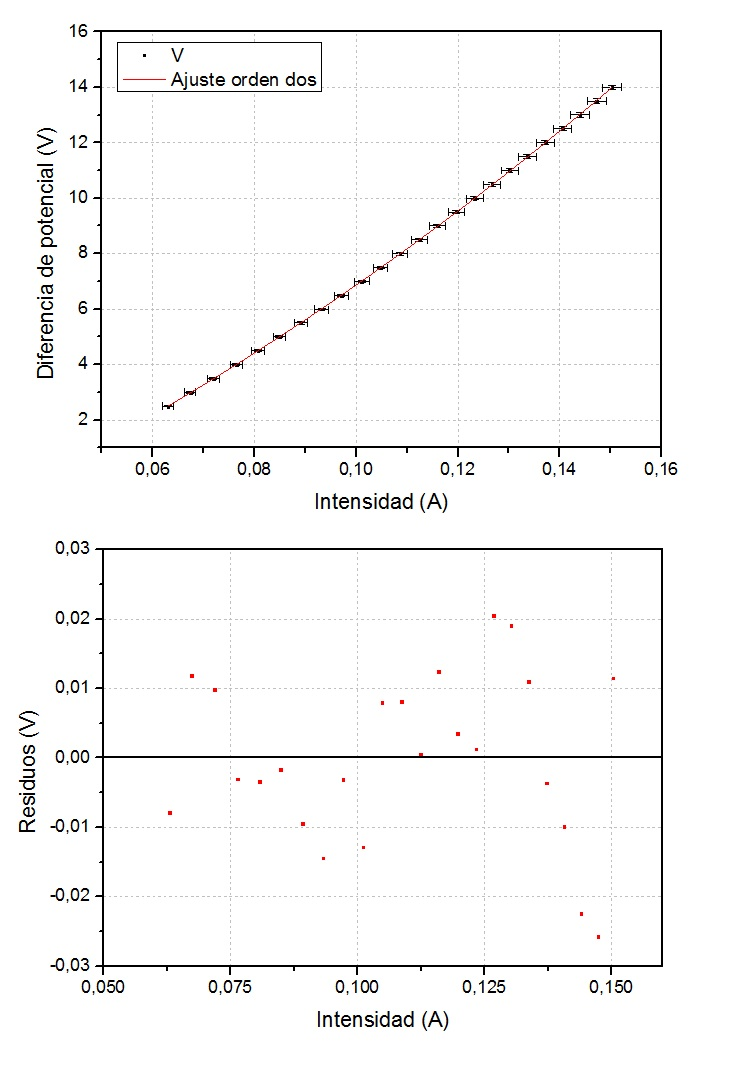
\includegraphics[width=\linewidth]{fig_o2.jpg}
\label{fig:o2}
\caption{Ajuste orden dos y sus residuos}
\end{figure}


%----------------ORDEN 3-----------------------------

El ajuste de orden tres tiene un gr\'afico similar al ajuste de orden dos y sus residuos tambi\'en son muy similares. El $R^2=0.99999$, como con el polinomio de orden dos por lo que ambos modelos explicaban el mismo porcentaje de los datos obtenidos. Su F=7E5, indicando como en el caso anterior que el hecho de que este ajuste sea aleatorio es improbable.\par

Sin embargo al observar los T-valores (Tabla \ref{tab:o3})para los distintos par\'ametros se puede notar que en este tercer ajuste, estos fueron considerablemente peores que en el anterior. En particular para el coeficiente c\'ubico se observa un bajo T-valor, lo que indica que este tercer par\'ametro tiene una baja significancia. Esto nos permiti\'o concluir que de los modelos utilizados, el que mejor caracteriza al sistema estudiado de la l\'ampara es el polinomio de orden dos con sus par\'ametros libres.\par

\begin{table}
\centering
\caption{Par\'ametros del ajuste de orden tres}
\label{tab:o3}
\begin{tabular}{|c|c|}
\hline
\multicolumn{2}{|c|}{$y(x)=ax^3+bx^2+cx+d$} \\ \hline
d                  & $-3.0\pm0.2$           \\ \hline
T-valor            & -19                    \\ \hline
c                  & $68\pm5$               \\ \hline
T-valor            & 13                     \\ \hline
b                  & $328\pm51$             \\ \hline
T-valor            & 7                      \\ \hline
a                  & $-191\pm164$           \\ \hline
T-valor            & -1.2                   \\ \hline
\end{tabular}
\end{table}

De esta forma podemos informar la resistencia din\'amica como:
\begin{equation}
\label{eq:resdin}
\frac{dV}{dI}=R(I)=(74.0\pm0.8)\Omega +(539\pm8)\frac{\Omega}{A}\cdot I
\end{equation}

%------------------------------------------------
%------------------------------------------------

\section{Conclusiones}


Comparando los valores obtenidos de la resistencia en los distintos ajustes (lineal, cuadr\'atico y c\'ubico), se encontr\'o que el modelo que mejor ajusta a los datos recolectados es el cuadr\'atico con origen forzado en cero. Esto esta de acuerdo con la bibliograf\'ia, ya que al ser el filamento de la l\'ampara incandescente un material no \'ohmico, su resistencia aumenta proporcionalmente con la ca\'ida de potencial debido al incremento de las colisiones entre las part\'iculas del filamento y los electrones al aumentar la temperatura de dicha resistencia (efecto Joule). En otras palabras, al aumentar la resistencia, se observa m\'as brillo en la l\'ampara.
\par 
Para realizar mediciones confiables, hubo que esperar cierto tiempo a que la temperatura del filamento se estabilice. Tambi\'en se tuvo en cuenta que las mediciones pueden ser afectadas por las resistencias internas del amper\'imetro y volt\'imetro utilizados



%----------------------------------------------------------------------------------------
%	REFERENCE LIST
%----------------------------------------------------------------------------------------

\begin{thebibliography}{99} % Bibliography - this is intentionally simple in this template

\bibitem{eq:potencial} E. M. Purcell, \textit{Electricidad y Magnetismo - Berkeley Physics Course Vol. 2}, Editorial Revert\'e S.A., 2da edici\'on, Barcelona (1988), p\'ag. 124
\bibitem{eq:ohm1} E. M. Purcell, \textit{Electricidad y Magnetismo - Berkeley Physics Course Vol. 2}, Editorial Revert\'e S.A., 2da edici\'on, Barcelona (1988), p\'ag. 124
\bibitem{eq:ohm2} E. M. Purcell, \textit{Electricidad y Magnetismo - Berkeley Physics Course Vol. 2}, Editorial Revert\'e S.A., 2da edici\'on, Barcelona (1988), p\'ag. 123
\bibitem{Fuente} http://www.hantek.com/Product/PowerSupply/PPS2320A.pdf
\bibitem{amp} https://www.scribd.com/doc/222262447/Manual-y-Diagrama-Esquematico-de-Multimetro-Digital-Protek-506
\bibitem{volt} http://www.ageta.hu/pdf/UT51-55.pdf
 
\end{thebibliography}

%----------------------------------------------------------------------------------------

\end{document}